\section{Task 3: Multisided Platform Mapping}
\label{sec:task3}





\subsection{Is it really a platform?}


A MSP is a multisided platform that lets two or more distinct groups interact directly, and each group is affiliated with the platform (Hagiu \& Wright, 2015). This test is important for S3NS. The core PREMI3NS looks like a pipeline. S3NS licences Google Cloud Technology, runs it in France under French control and sells capacity to clients. If that were S3NS would be a sovereign reseller, not a platform. 

We argue that PREMI3NS is a hybrid. The pipline part bring in the most of the revenue, but there is a platform laywe on top of it. S3NS presents its offer as an ecosystem where service partners help clients migrate, and independent software vendores, ISVs ass their own solutions on top of the cloud (S3NS, n.d-a). The clearest example is SAP. In 2026 SAP agreed to run its RISE private cloud ERP on PREMI3NS, with commercial availability planned for the second part of 2026 (Thales, 2026a). SAP joins to reach regulated clients it could not otherwise serve, and clients join partly because software like SAP is available inside the trusted perimeter. The value each group gets depends on how many members the other group has. That is the defining feature of MSP (Rochet \& Tirole, 2003; {\0}verby \& Audestad, 2021)}.

Two actors oftenly are wrongly treated as platform sides. Google for instance is not a side. It only supplies the technology to the aliances and is paid for that, but google do not transact with clients through the platform. ANSSI isnt a side either, it only sets the rules that decide who may enter the trusted perimeter at all. Both shape the platform from outside the market it creates. 

\subsubsection{The sides}

\textbf{Side 1: Client institutions.} This side is divided into two groups with their own need. The first is French state administration. When they host sensitive data with an external cloud provider, they must use a SecNumCloud qualified service. That rules started off as the government's "cloud au centre" doctrine and was written into law through the 2024 SREN law, with implementing rules adopted in 2026 (Acteurs Publics, 2026; ANSSI, n.d.). The second group is are large companies in regulated sectors. Around ~30 early adopters tested the PREMI3NS before qualification, and EDF and Thales itself are name users (S3NS, 2025). For these firms, trusted cloud is a strategic choice and not a legal duty. Both groups face high switching costs once they have migrated.

\textbf{Side 2: Complementators}. These are ISVs, SaaS providers and service partners (integrator and consultancies). They must have invest to port to qualify their products, and most can also offer them on competing trusted clouds, so they multi-home. An industry analysis describes the ISV model on PREMI3NS as still at an early age (Futurm Group, 2026). This means the platform does not yet have a large complementor side, which is exactly the chicken-and-egg problem MSP theory describes.


\begin{figure}[H]
    \centering
    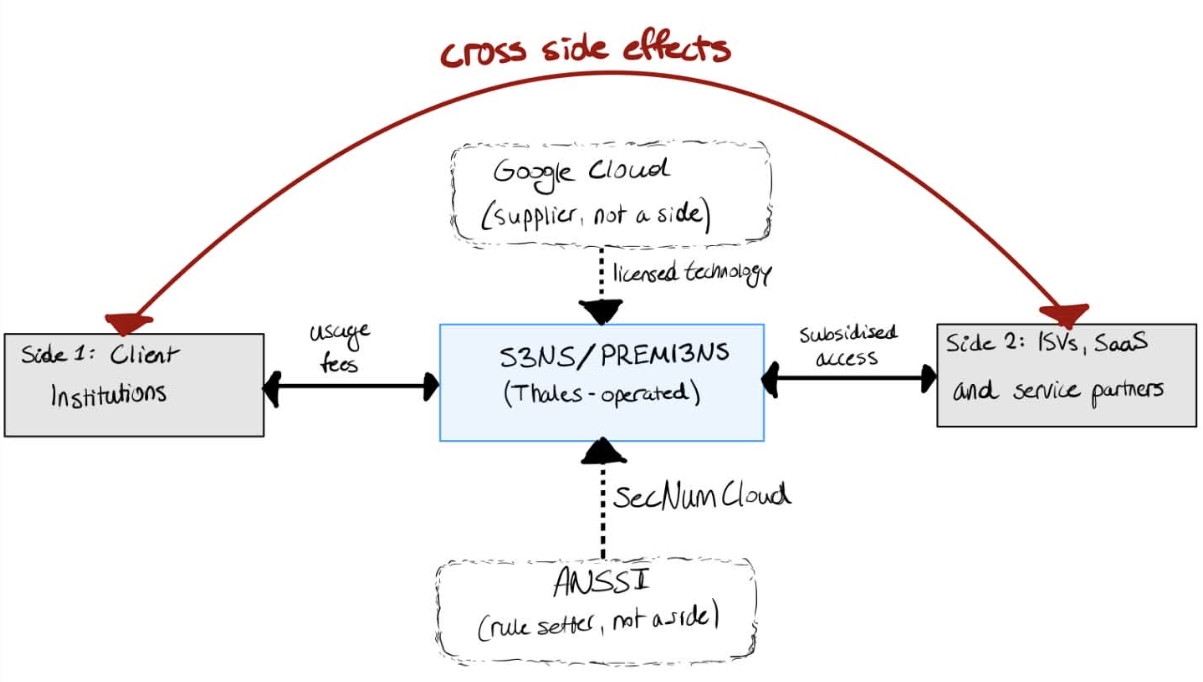
\includegraphics[width=0.90\linewidth]{55555.png}
    \caption{Multisided Platform Map of PREMI3NS. Solid lines are platform sides, dashed lines are suppliers and regulators outside the platform market}
    \label{fig:msp}
\end{figure}

\subsubsection{Cross-side and same-side effects}

The table ~\ref{tab:effects} summarises the effects. The strongest effect runs from the clients to the vendors. Every new regulated client makes the market for SecNumCloud ready software larger and before the qualification this market barely existed. The effect from vendors to the clients is positive but weaker. A client can only move a workload if the software it needs is available, as the SAP case shows for the ERP systems. However, many clients build their own applications directly on the infrastructure, and the Google compatibility means familiar tools are already there. 

The same side effects are weak. Among the clients, early adopters create reference cases and experience that others copy. As the section~3.2 argues for, this is mostly a learning effect and not a true network effect. A ministry does not gain directly because another ministry join. Among vendors, the same-side effect is mostly negative, since they compete for the same small group of clients. 


\begin{table}[h]
\centering
\begin{tabular}{|p{3.3cm}|p{1.4cm}|p{8.3cm}|}
\hline
\textbf{Effect} & \textbf{Strength} & \textbf{Reason} \\ \hline
Clients $\rightarrow$ Vendors & High & New regulated clients open a market that vendors cannot otherwise reach. \\ \hline
Vendors $\rightarrow$ Clients & Medium & More workload can migrate, but many clients build their own applications \\ \hline
Client $\leftrightarrow$ Client & Low (+) & Learning and reference cases, not direct network value \\ \hline
Vendor $\leftrightarrow$ Vendor & Low ($-$) & Competition for the same clients, some shared skills and tools \\ \hline
\end{tabular}
\caption{Cross-side and same-side effects on PREMI3NS (qualitative assessments)}
\label{tab:effects}
\end{table}

\subsubsection{Pricing Architecture}

MSP Theory states that the platform should subsidise the side that is more price sensitive and creates more value for the other side, and it should charge the side whose demand is less elastic (Rochet \& Tirole, 2006; Parker \& Van Alstyne, 2005). A new platform must also get one side on board first to solve the chicken-egg problem (Caillud \& Jullien, 2003). 

The client side is partly documented. S3NS published a catalouge price list in euros. Each service is billed per unit used, for instance per vCPU hour or per gigabyte per month. Many serivces offer a free usage tier, and clients who commit for one or three years get lower unit prices  (S3NS, n.d.-b). For a standard C3 compute core, the one-year price is about 28\% lower and the three-year price about 46\% lower than the pay-as-you-go price. This confirms that the clients are the money side. It also shows a pricing tool that matters for Section~3.2. The commitment discount trades a lower-price today for a longer tie to the platform, so it strengthens lock-in. Clients with sensitve data accept this because the law and the small number of qualified providers make their demand less price elastic. Private firms have more choice, and negotiated commitments let S3NS offer them a lower effective price than state buyers who have to use a qualified cloud. 

the complementor side is not documentes, so we build it from theory. Since the ISV part is still small (Futurm Group, 2026) and vendors multi-home, they should be subsidised through low or zero platform fees, technical help with porting and support toward qualification (A2). The SAP deal shows another kind of subsidy. Thales, one of the alliance partners, became the first customer of SAP on PREMI3NS (Thales, 2026a). This guaranteed demand lowers SAP's risk of joining. The alliance uses one of its own partners as an anchor client to attract the other side. 

Table~\ref{tab:pricing} summarises the architecture.


\begin{table}[h]
\centering
\begin{tabular}{|p{2.6cm}|p{2.2cm}|p{4.6cm}|p{3.6cm}|}
\hline
\textbf{Side} & \textbf{Role} & \textbf{Instruments} & \textbf{Basis} \\ \hline
Sate administrations & Pays & List prices, commitment discounts & Price list; legal duty \\ \hline
Regulated Firms & Pays (less) & Negotiated commitments, free tiers & Price list; theory \\ \hline
ISVs and service partners & Subsidised & Low fees, porting help, anchor demand & Theoru; SAP case \\ \hline
\end{tabular}
\caption{Pricing Architecture of PREMI3NS}
\label{tab:pricing}
\end{table}

These prices are likely to change over time. Once clients are locked in a single-home for each workload (A4), competitive bottleneck theory predicts that the platform controls access to them and can start charging the multi-homing side (Armstrong, 2006). S3NS could then introduce fees for listing and certifying vendor solutions. The vendor subsidy is therefore likely to be temporary. 

the alliance structure decides who fund the subsidy. Client revenue flows to S3NS, and part of it goes to Google as licence fees (A3). Google therefore shares in the growth of the paying side, while the cost of subsidising vendors falls mostly on Thales, through S3NS and through its own role as anchor client. At the same time, software built for PREMI3NS uses Google technology, so google gains from the subsidy without paying for it. This uneven split is a real tension inside the alliance. It also matters for Section~4.2, because the clients who pay are the ones who carry most of the loss is the platform is breached. 

\subsubsection{Assumptions}

\begin{description}
  \item[A1.] PREMI3NS unit prices include a premium over standard Google Cloud prices for compareable services. We did not compare the two price lists line by line. The assumption rests on the extra cost of sovereign operation: separate infrastructure, French staff and quarantine zone where every Google update is checked before use (S3NS, 2025).
  \item[A2.] Vendors are price sensitive and multi-home. The ISV model is still young (Futurm Group, 2026), and vendors can also qualify their products on competing trusted clouds.
  \item[A3.] Google is paid through the licence fees that grow with usage. The contract is not public, If the fee were fixed instead, Thales would carry all the volume risk. 
  \item[A4.] After migration, each client workload effectively single-homes, because of the switching costs identified in Section~3.2 and the multi-year commitments in the price list.
\end{description}

